%\required{Project Summary}

%\newpage
%\setcounter{page}{1}

\required{Project Description}

\section{Introduction} % start page 1 % Galaxy Surveys are great 
Spectroscopic galaxy surveys play an indispensable role in precision cosmology.
The measurements of the Baryon Acoustic Oscillation (BAO) peak position at
various redshifts put tight constraints on the expansion rate and geometry of
the Universe. The Redshift-Space Distortion (RSD) signal, which has its origins
in the growth of structure over cosmic time, can constraints the growth rate as
well as a function of redshift. These measurements have been
pushed to a very high precision. BAO are now measured at a one per cent
precision,  while the best RSD measurements stand at about a five per cent
precision. The next generation of galaxy surveys, such as Dark Energy
Spectroscopic Instrument (DESI), Euclid satellite mission, and the Wide Field
Infrared Survey Telescope (WFIRST), will extend these measurements to higher
redshifts and even better precision.

% Dark Energy gravity still unclear close to LCDM and GR 
When these measurements are combined with a Cosmic Microwave Background (CMB)
data the resulting constraints on Dark Energy (DE) and theories of gravity
(TG) are overall consistent with the standard cosmological $\Lambda$CDM model.
The constraints however at this point are not tight enough to conclusively rule
out alternative models of DE and TG that are arguably better motivated from a
fundamental physics point of view than the standard cosmological model. In
addition, there are a number of 2 to 3 $\sigma$ discrepancies (such as e.g.
the discrepancy with the local Hubble constant measurements, or the tension
with the clustering amplitude measured by weak lensing surveys), but they are
not statistically significant enough to make a conclusive case in favour of
non-standard models.
 
% There will be a cosmic variance limit for standard analysis 
Since we have only one vintage point for observing the Universe the amount of
information that is  available to us is fundamentally limited. Both BAO and RSD
tests, as currently implemented, rely on two-point statistics measurements of
the galaxy field the precision of which is limited by the total  observable
volume.  Expected DESI data will almost saturate this ``cosmic variance'' limit
at lower redshifts where DE dominates the evolution. Hopefully, we will be able
to either strongly rule out alternative scenarios or find a convincing
non-$\Lambda$CDM signal. If we, however, end up with a number of nagging
discrepancies that are suggestive but not statistically significant, the only
way to resolve the issue will be to find an alternative source of robust and
precise cosmological constraints in the same data.

% We need to squeeze out more information 
There are a number of ways to extract more information from spectroscopic
galaxy data. We can try to enhance the standard BAO analysis by (by now
standard) method of reconstructing the linear field or trying to come up with
more optimal weighting schemes. Other approaches include looking at stacked
voids, joint multi-tracer analysis, and going to smaller scales by means of
simulation assisted modeling. All these approaches have their advantages and
disadvantages and all of them must be tried out on real data. In this proposal
we would like to pursue the same goal by going to the third-order statistics of
galaxy fields.

% what we propose, what we ask for 
The main objective of this proposal is to develop methods for
\textbf{extracting robust BAO and RSD measurements from the  bispectrum of
galaxies on linear and semi-linear scales}. We argue that, even though this is
a difficult  endeavour that has a number of inherent risks, it also has a
number of potential advantages over alternatives (e.g.  using a two-point
statistics of reconstructed fields, or extracting RSD signal from stacked
objects such as stacked voids), and is worth pursuing. The main appeal of
bispectrum is that, at least for some future surveys, it has a potential to
\textbf{significantly enhance} the standard BAO/RSD analysis. We hope to
convince our colleagues that the benefits outweighs the risks and this line of
research merits a modest investment of resources and that our preliminary work
this direction places us in a good position  to perform this research. 

% end page 1

\section{Bispectrum overview}

% 2pt and 3pt 
Spectroscopic galaxy surveys provide us with highly accurate measurements of 3D
positions of millions of galaxies in large cosmic volumes.  The specific
distribution of galaxies that we observe is just one out of a large number of
possible distribution that could have been observed in the same cosmological
model if the stochastic initial conditions were slightly different. The most
popular way of describing this stochasticity in the large-scale structure
community has been to use the n-point correlation functions.  The two-point
correlation function $\xi(\vec{r})$ is a function of a separation vector
$\vec{r}$ and describes a ``clustering strength'' at a certain scale (average
number of neighbours at distance $\vec{r}$ from a randomly selected galaxy in
access of a purely random distribution).  Three-point function $\eta(\vec{r}_1,
\vec{r}_2)$, similarly, describes a probability of finding three galaxies  in a
specific triangular configuration.  This information is sometimes expressed in
terms of Fourier transforms of these two functions  (power-spectrum
$P(\vec{k})$ and bispectrum $B(\vec{k}_1, \vec{k}_2)$ respectively). From now
on we will use the term ``bispectrum'' to generically refer to the three-point
function both in Fourier and configuration spaces. 

% How is 3pt generated 
For purely Gaussian fields the two-point statistics contains all of the
information and the expectation value of bispectrum is zero.  Even though the seed
cosmological fluctuations are believed to be very close to Gaussian
gravitational instability and halo/galaxy bias generate non-zero bispectrum at
late times. Non-linear terms in the Euler equation will inevitably
couple initially independent Fourier modes and will therefore generate
bispectrum. The relationship between DM and galaxy overdensities  is linear
on very large scales but non-linear and non-local effects become more important
on smaller scales. Because of this non-linear mapping the galaxy distribution
would have a non-zero bispectrum even if it was generated form a purely
Gaussian DM field. This immediately suggests that bispectrum should be
sensitive to the exact nature of TG and higher order bias parameters.
\textbf{We will later argue that the sensitivity to DE  through projection
effects is even stronger.} Planck data put very tight upper limit on local
primordial non-Gaussianity parameter -- $f_\mathrm{nl}$ -- at least for some
triangular configurations. This is not a problem for our research program since
we do not intend to use bispectrum as means to measure $f_\mathrm{nl}$, in fact
the small value of $f_\mathrm{nl}$ makes the modeling part significantly
easier. Our goal is to measure BAO/RSD from the distortions of the bispectrum
shape and as we will later show for this goal the bispectrum generated by
gravitational instability and higher order bias is sufficient.

% What does 3pt look like 
The measured bispectrum is a function of of five variables: three variables describing the size of the triangle (e.g.
wavelengths $k_1, k_2, k_3$ corresponding to three sides) and two variables
describing its orientation with respect to the line of sight (e.g. angle that
one of the sides makes with respect to the line of sight, and the internal
rotational angle of the triangle). The potential to constrain cosmological
parameters comes from the fact that the exact shape of this  five dimensional
function depends on initial conditions, the nature of gravity that generated
it, and the higher order bias. The accuracy of bispectrum measurements is
related to the number of independent galaxy triangles in the survey. The
dominant contributions to the uncertainty in measured bispectrum come from
``cosmic variance'' and ``shot-noise''. Shot-noise stems from the fact that
sparsely sampled galaxy populations have smaller number of triangles and for
the bispectrum (assuming Poisson distribution) scales as  $1/n^2$, where $n$ is
the number density of galaxies. The cosmic variance scales as $1/V$ with the
survey volume and reflects the fact that larger volumes have more independent
triangular configurations. Large scale measurements are limited by the cosmic
variance and small scale measurements by the shot-noise. The overall variance
of the bispectrum measured in wavevector bins scales as (up to a normalization
factor, and under a number of simplifying assumptions)  

\begin{equation}
\mathrm{Var}\left[B(\vec{k}_1,\vec{k}_2,\vec{k}_3)\right] \propto
\frac{k_1k_2k_3\Delta k_1\Delta k_2\Delta
k_3}{V}\left[\frac{P(\vec{k}_1)P(\vec{k}_2) + P(\vec{k}_2)P(\vec{k}_3) +
P(\vec{k}_3)P(\vec{k}_1)}{n} + \frac{1}{n^2}\right], 
\end{equation} 

where $\Delta k$-s are the widths of wavevector bins. For comparison the power
spectrum variance scales as 

\begin{equation}
\mathrm{Var}\left[P(\vec{k})\right] \propto \frac{k^2\Delta
k}{V}\left[P(\vec{k}) + \frac{1}{n}\right].  
\end{equation}  

This rough comparison demonstrates that the signal to noise of measured
bispectrum benefits much more from increasing sampling density  compared to
the power spectrum ($n^{-2}$ vs $n^{-1}$). It also benefits much more by
extending the analysis to smaller scales (higher wavenumbers, $k^6$ vs
$k^3$). So, the higher the number density is and simpler the non-linear
modeling is more competitive the bispectrum constraints become. Our forecasts
suggest that, if we manage to control systematic effects, bispectrum is capable
of delivering impressively competitive constraints for DESI Bright Galaxy
Survey (BGS) and the lower redshift range of WFIRST. Both of these samples have
a high number density and WFIRST is additionally at a high redshift (hopefully
allowing to push the analysis to higher values of $k_\mathrm{max}$). The
projected bispectrum constraints from DESI main samples and Euclid are also
very interesting.

\section{BAO/RSD analysis}

The primordial shape is imprinted very cleanly in the initial distribution.
Later gravitational evolution mixes the modes and moves some of the shape
information from power spectrum to bispectrum. If cosmological constraints
were coming \textbf{only from the initial shape} contribution of bispectrum to
the power spectrum would be modest. Reconstruction of the initial
linear field would then move all of this higher order information back to the
power spectrum. Fortunately, we have other effects in the observed clustering
that are \textbf{far more sensitive to DE and TG then the initial shape}. Most
of the BAO constraints on DE actually come from so called Alcock-Paczynski (AP)
distortions of the feature rather than actual determination of its physical
scale. Similarly, most of TG constraints come from radial RSD signal.

% BAO/RSD in general 
BAO is a preferred scale set by processes in yearly Universe. It manifests
itself as a peak in the correlation function and an oscillatory pattern in the
power spectrum. The BAO scale has been measured with an exquisite precision by
CMB experiments and convincingly detected in low redshift galaxy samples. Since
baryonic matter only comprises a small fraction of non-relativistic matter, the
BAO feature is not as strong in galaxy distribution as it is in CMB. \textbf{The
constraining power of the BAO in galaxy distribution is strongly enhanced by
the AP effect}. The AP effect results from the fact that we observe galaxies in the space of
angular coordinates and redshifts. To link these  to theoretical  predictions
we need to translate them into physical distances. To do this we need to know
the angular diameter distance $D_A$ (for angular distances)  and the Hubble
parameter $H$ (for radial distances) at the redshift of our galaxy sample. If
we pick wrong $D_A$ and $H$ our scaling will be off. Since we know the
position of the BAO peak at a very high precision from CMB data, we can use AP
distortions to find a correct value of $D_A$ that aligns BAO in galaxy
distribution with the correct physical scale. Performing this alignment in the
radial direction similarly constraints $H$. These $D_A$ and $H$ measurements
can then be translated into strong and robust DE constraints. In principle, AP
effect would work even without the BAO feature, but the presence of a well
calibrated peak (or for the power spectrum oscillatory pattern with known
frequency) makes it easier to detect small shifts.

RSD is an anisotropic signal in the galaxy distribution that results from the
fact that galaxies on average tend to fall into each other and because of this
coherent extra Doppler shift their radial distances seem on average to be
smaller than they really are. Since we belie that there is no fundamental
reason for galaxy distributions to have a different statistical pattern in
radial and angular directions, we can use measured RSD to constrain infall
velocities of galaxies. And since gravitational interactions source the infall
velocities this information can then be translated into strong constraints on
TG.

BAO are considered to be very robust and virtually systematics free
measurements. RSD modeling is more involved and significant systematic effects
can be present already on semi-linear scales. There is no straightforward way
of isolating the RSD feature in the analysis, so the RSD measurements must
always incorporate AP measurements on the full power spectrum shape. However,
if the systematics can be brought under control RSD enhance the constraining
power of galaxy surveys by an order of magnitude, and make it possible to
constrain TG in addition to DE.

% BAO/RSD in 2pt 
Our flagship BAO/RSD measurements have so far come from two point statistics.
The BOSS measurement is so far the most accurate (1\% at $z\sim0.57$).
Large-scale BOSS measurements stand at 5\%.  DESI, Euclid, and WFIRST are
projected to make multiple similar sub-percent level measurements up to a
redshift of $z\sim 2$.

% BAO/RSD in 3pt 
The full fledged equivalent BAO/RSD bispectrum measurements on linear and
semi-linear scales have not so far. Early works have been mostly concerned with
the small scale bispectrum with the purposes of estimating bias parameters.

\section{Bispectrum projections}

% Forecasts are good  
\begin{wrapfigure}{r}{0.5\textwidth}
\begin{center}
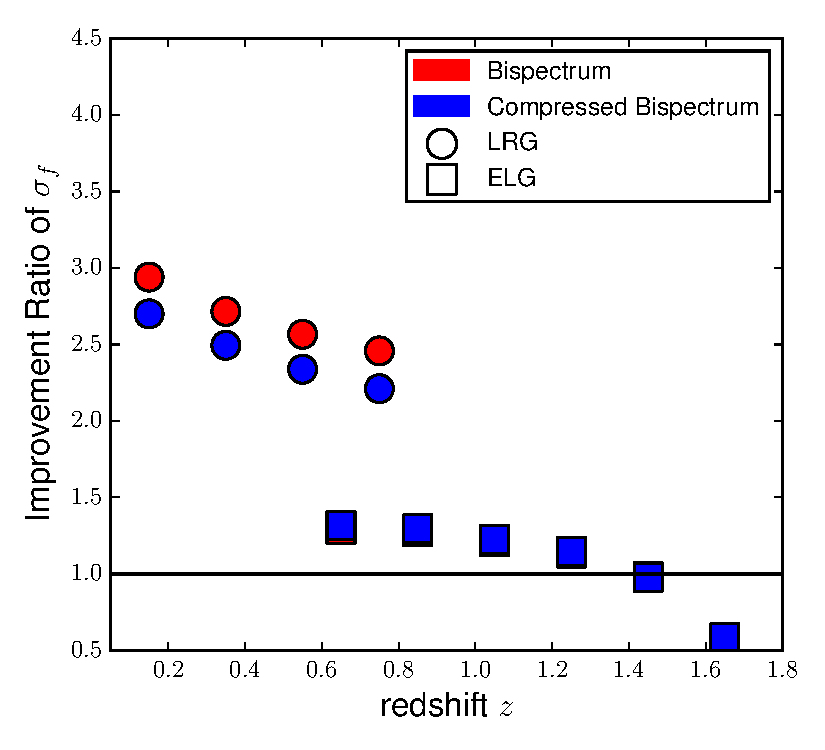
\includegraphics[width=0.48\textwidth]{fz.pdf}
\end{center}
\end{wrapfigure}


% Let's do forecast 
At this point, it would be interesting to check how much cosmologically
relevant information is in the potential bispectrum measurements from future
surveys. We expect bispectrum to perform well on densely sampled surveys (e.g.
DESI BGS or low-redshift WFIRST). We use conventional Fisher information matrix
techniques to perform these forecasts. We assume that bispectrum is analysed in
exactly the same way as the full BAO/RSD power spectrum analysis, i.e. it is
measured in bins that are narrow enough not too loose a lot of information to
in-bin averaging, the nonlinear effects are separated by choosing a value of
$k_\mathrm{max}$ appropriate for each redshift (more scales are included for
higher redshifts), uncertainties in the DM to galaxy biasing and intra-halo
motions are parametrized by bias parameters and a fingers of god dispersion
term. The parameters of interest are the two AP distortion parameters that
correspond to $D_A$ and $H$ and an RSD parameter ($f\sigma_8$) that can be
related to the growth rate.

Figure above shows such prediction for $f\sigma_8$ parameter for DESI
survey divided in redshift bins of $\Delta z \sim 0.1$. Plotted is the ratio of
variance from power spectrum to that of the bispectrum. It is interesting and
encouraging to see that the bispectrum analysis outperforms the standard power
spectrum in this regime by almost a factor of 3! At higher redshifts the
improvement is more modest but even there the bispectrum RSD constraints are
comparable to the ones derived from power spectrum. It is worth highlighting
that these predictions are for the bispectrum only. Combining $P(\vec{k})$ and
$B(\vec{k}_1,\vec{k}_2)$ Fisher matrices is complicated because of the presence
of cross-correlation terms and we currently do not have a reliable code to
perform these computations. Nevertheless, it is clear that the addition of the
bispectrum would strongly enhance overall constraints even after-accounting for
the cross-correlations (Our mock tests suggest a cross-correlation of about 30
per-cent, consistent with findings of Ref.~[]). We see similar improvements for
BAO measurements and for Euclid and WFIRST samples.

\section{Bispectrum advantages}

In this section we will compare bispectrum analysis to alternative ways of
extracting extra information from galaxy surveys on top of standard two-point
BAO/RSD. The intent here is not to argue that the bispectrum approach is
superior but rather to show that despite its intrinsic difficulties it has
advantages that merit further development and research.

% Bispectrum over improvements
A safe option (one that is not likely to introduce additional systematics) for
improving standard BAO/RSD measurements is to implement weighting schemes that
are in some ways more optimal than the standard Feldman-Kaiser-Peacock
prescription. Weighting schemes based on relative bias of galaxy sub-samples
and redshift evolution have recently been studied in literature. Even though
they have a potential to somewhat improve the measurements they could never
achieve a factor of three improvement that is potentially present in the
bispectrum.

% Bispectrum over reconstruction
A very popular methods, that has by now become standard, is to undo some of the
effects of non-linear evolution on large scales by reconstructing the initial
field. This sharpens the power spectrum shape around BAO and makes it more
sensitive to the AP test (sensitivity to small distortions scales as
$\mathrm{d}P/\mathrm{d}k$ to leading order). The effectiveness of
reconstruction is limited by two factors. At high redshifts the BAO shape is
closer to linear and there is not much to gain by making it sharper. Also, it
is not completely clear how the reconstruction interplays with RSD. Even though
it is possible to run a reconstruction algorithm without removing RSD signal,
some kind of RSD modeling will have to be adopted, and it is not entirely clear
that this procedure will not bias the extracted RSD constraints. Reconstruction
is therefore suitable for BAO only constraints but does not help with the RSD
analysis.

Bispectrum is an independent (although somewhat correlated) measurement that
can be used for the BAO/RSD measurements. Small distortions in the
bispectrum shape can be used to constraint $D_A$ and $H$ in a way that is
identical to the power spectrum (even if the modeling of former can be more
complicated). While reconstruction linearises BAO peak in power spectrum it
also reduces the bispectrum amplitude. For the number densities that are
typical for current surveys (order of $10^{-4}\ \mathrm{Mpc}$/h) the gain in
the power spectrum sensitivity to AP is approximately equal to the loss in the
bispectrum sensitivity. For current surveys this implies that the BAO
constraints from reconstructed power spectrum are roughly equal to the kind of
constraints that are obtainable from a joint power spectrum and bispectrum
analysis, and since the former is simper there is no convincing case for the
later. This is not however true at higher densities and higher redshifts where
the sharpening of power spectrum BAO feature does not gain as much information
as adding a bispectrum function to the analysis. 

In summary, \textbf{the information content of reconstructed power spectrum is not
always equal to the information content of joint power spectrum and bispectrum
(plus higher order correlators) analysis}. They would be equal for a field in a
box, where the shape of the power spectrum of initial nearly Gaussian field
contains all the information and gravitational evolution only serves to couple
the phases and dilute this information into higher order terms. Our constraints
however are coming from AP distortions of observed quantities and having an
extra distorted function (bispectrum) is in some cases more profitable than
having a slightly ``sharper'' power spectrum. \textit{This is easy to see for a
hypothetical case of a universe without a BAO feature (perhaps a Universe with
trace amounts of baryonic matter). In that universe reconstruction would not
really add anything to the power spectrum, it would simply slightly tilt the
power law. But having an extra function (bispectrum) for the AP analysis would
obviously increase the constraining power.}

% Bispectrum over voids
Another popular technique for going beyond standard BAO/RSD analysis is to use
stacked voids (or clusters) that are assumed to be isotropic in physical space
because of the statistical homogeneity. The observed anisotropies than are
generated by AP and RSD and can be used to obtain DE and TG constraints. The
method has a huge statistical promise, the number of objects after all scales
linearly with volume. The main challenge is the modeling. Voids (and clusters)
are small scale objects that are strongly affected by non-linear evolution and
do not lend themselves to perturbative treatments like large scale n-point
statistics do.

% Bispectrum over small scale
Yet another extremely promising option is to use statistical measures on small
extremely non-linear scales. These scales are too non-linear to be modeled from
first principles and therefore theoretical modeling will have to be aided by
high quality and resolution cosmological simulations. The main question is
whether we will in fact have suitable (in terms of quality and numbers)
simulations that are accurate enough for this purpose, large enough to have
appropriately small errorbars, and diverse enough to meaningfully cover large
parameter space which, in addition to cosmological parameters, should now
include extra parameters describing small scale physics (Halo-galaxy connection
parameters, baryonic effects, environmental effects, etc.), \textbf{in time for
DESI/Euclid/WFIRST analysis.}

% All must be tried
All these are excellent ways of significantly enhance cosmological information
coming from spectroscopic galaxy surveys, and the entire community hopes that
they will all be mature enough in time to be applicable to DESI/Euclid/WFIRST
data.  They should all be pursued to make sure that we have multiple
complementary ways of looking at the data and spot possible systematics. It is
clear that BAO/RSD from bispectrum on linear and semi-linear scales has it's
role in this joint effort. Some potential advantage are that, unlike voids, the
modeling is bound to work at least on extremely large scales where the
perturbative approach will eventually work (the real question is how far we can
slides this boundary down the scale ladder); Unlike small scale clustering the
modeling will not rely as much on simulations (although the validation most
definitely will, and some calibration on simulations may be necessary); And
compared to reconstruction it has a theoretical potential to deliver
significantly stronger enhancements.

\section{Bispectrum -- Status Quo}

% previous works
Early bispectrum measurements in galaxy distribution have been made in
(exhaustive list of early works here with short description).

% BOSS and WiggleZ work
More recent bispectrum measurements have been performed in WiggleZ and BOSS
galaxy samples. 
% our work
\begin{wrapfigure}{r}{0.5\textwidth}
\begin{center}
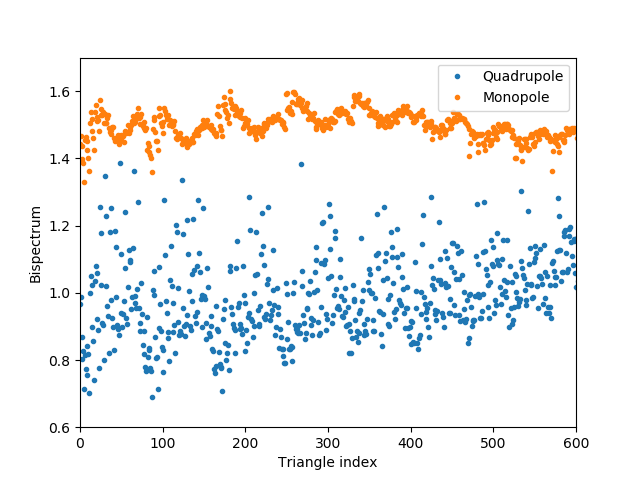
\includegraphics[width=0.48\textwidth]{MonQuad.png}
\end{center}
\end{wrapfigure}
Our group has published a number of recent papers related to galaxy bispectrum
analysis. In Ref.~[] we studied the ways of reducing bispectrum information
without sacrificing information content and identified three harmonic angular
modes that contain most relevant information. In Ref.~[] we detected a BAO
signature in BOSS CMASS bispectrum monopole. Our measurement was systematics
limited but still allowed us to convert the measurements to a 2 per cent
distance measure. We showed on the mocks that a systematics free measurement
would be slightly tighter compared to the one obtainable from the reconstructed
power spectrum. We are currently working on extending our work to anisotropic
bispectrum analysis. This will allow us to constrain both angular and radial
BAO parameters. Preliminary MCMC chains from this measurement are displayed on
Figure~2. Our proposed work would take over from here and would add RSD to the
mix. We will also work on a more careful study of possible theoretical and
observational systematic effects to bring the errorbars down.


\section{Research Plan}

% What we will do
Our overall goal is to develop methods of measuring BAO and RSD in large-scale
bispectrum of galaxy surveys. Achieving this goal schematically involves five
steps: measuring bispectrum, estimating covariance matrices, modeling or
removing observational systematics, theoretical modeling, and likelihood
analysis. Our tentative plans for each of these directions are briefly
described below.

\subsection*{measurements}

The bispectrum measurements are generally more difficult and computationally
demanding than the power spectrum measurements. Fortunately, recent
developments have made this task significantly easier. Recent works have
demonstrated that even wide-angle bispectrum measurements can be reduced to a
series of Fast Fourier Transforms (FFT), and that the triangle counting can
also be reduced  to a combination of FFTs and convolutions. Our group has
developed a fast GPU implementation of bispectrum multipole algorithm that has
been validated on controlled mocks and can process order of few thousand mocks
(of the size of BOSS CMASS sample) in order of few hours.

This part of the work will be concerned with further high precision testing of
our pipeline. We will produce particle distributions with known input power
spectrum and bispectrum following e.g. Ref~[]. We will then check that our
pipeline accurately reproduces the input. To accomplish this task we will not
need to evolve the initial conditions under gravity, which will make the task
computationally inexpensive. 

In addition, we will test methods of modeling the shot-noise and window effects
on the measurements. We expect the simple Poisson shot-noise model to work
sufficiently well on large scales but this expectation will be tested on
controlled simulations. In previous works the window effects have either been
ignored or modeled in an ad-hoc way. Exact window convolution for bispectrum
requires computing a six-dimensional double convolution integrals which is
computationally challenging, especially considering the fact that the
convolution will have to be performed for every model in Monte Carlo Markov
Chains. We will investigate approximate methods that are accurate enough for our
purposes and fast enough to be implement in the likelihood pipeline. 

Another topic that we will look into is related to the optimal reduction of
bispectrum data. Measuring bispectrum monopole and quadrupole in fine
wavelength bins will result in a very big data vector. This may prove
problematic at a later stage for estimating covariance matrices. There are
multiple possible ways of reducing the data vector size. One possibility is to
identify the triangular shapes that carry the most information on BAO/RSD and
remove the others. A more elaborate method along these lines would consist of
identifying the most informative linear combinations of bispectra bins. We will
explore all these options and will check how well they perform.

\subsection*{covariances}

The covariance matrices of measured bispectra provide another challenge. The
standard method of estimating covariance matrices from a sample variance of a
large number of mocks is complicated by the fact that there are a very large
number of bins and an accurate estimation of covariance and precision matrices
will require a large number of mocks. This problem becomes even more acute for
a joint power spectrum and bispectrum analysis. The covariance matrices in this
case are large and clearly non-diagonal.

We plan to tackle this problem from two complementary directions. One is to
somehow reduce the size of data vector so that computing covariances from the
mocks becomes a possibility. Another route is to estimate covariances at least
partially theoretically and calibrate theoretical estimates with mocks. 

% reducing size
Ref.~[] showed that it is possible to compress measured bispectrum to a
significantly smaller vector without loosing too much information. This
approach is very effective but requires the knowledge of covariance matrix and
is model dependent. Other approaches include further reduction of bispectrum
multipoles into e.g. first few multipoles in triangular configuration angle, or
identifying few principal components and only using them in the analysis. All
these approaches can be tested in a straightforward manner on mocks.

% theory
The exact theoretical estimation of bispectrum covariance would require
computing a six-point function and is probably an unachievable goal. It is
however likely that, especially at high redshifts, the covariance is dominated
by the leading order terms which are reasonably easy to compute. The biggest
effect would than be the effect of the mask on covariance and the coupling
between shot-noise and mask effects. We will borrow some recent ideas that were
demonstrated to work for the power spectrum (Refs.~[]) and will generalize them
for the bispectrum while making additional simplifications (e.g. assuming that
the bispectrum window function isotropic). Taking into account the fact that
fractional error in bispectrum in individual bins is lower than for the power
spectrum and that our requirement on the accuracy of covariance matrix is not
as stringent as a similar requirement on the model, we will identify
approximations that are good enough for our purposes and do not bias likelihood
fitting strongly. We can then use methods such as shrinkage to combine our
theoretical covariance with the sample variance. For this approach to work we
do not really need parameter free covariance matrices. Presence of few extra,
physically motivated, parameters would be acceptable and they would later be
calibrated on simulations.

\subsection*{observational systematics}

All observational systematics affecting the standard two-point BAO/RSD analysis
are also likely to affect the bispectrum. Most observational systematics affect
one point distribution (e.g. certain areas of sky have a lower efficiency of
having galaxies detected or the efficiency is a function of emission line
flux). These systematic inefficiencies are usually expressed either in terms of
visibility cubes (implemented in practice as random catalogs) or as sets of
per object weights. The mitigation of observational systematics is a very high
priority task for DESI/Euclid/WFIRST collaborations. We will closely follow
this work (PI Samushia is actually involved with some of this work) and will
implement the known mitigation techniques in our bispectrum analysis. It is
difficult to imagine observational systematics that would be either exclusive
to the bispectrum or significantly more severe.

% bitwise weights
There are some systematics that may not directly translate from the power
spectrum analysis and may require a separate investigation. These are the
systematics that affect the configuration space and can not be split into a
product of one-point weights. A good example of this type of systematics is
e.g. fiber assignment effects in DESI and slitless-spectroscopy effects in
Euclid.

Two proposed methods of dealing with fiber assignment effects are to remove the
most affected modes or to use a pair-wise weighting. Even though the power
spectrum specific versions of these methods can not be directly applied to
bispectrum they can be easily generalised. It should be reasonably
straightforward to identify the most affected bispectrum configurations and to
exclude them from the analysis. It should also be reasonably straightforward
to generalise pair-wise weighting schemes to triplet-wise weighting. In fact,
the bit-wise weights as implemented in Ref.~[] can be very easily translated
into triplet-wise weights.

In summary, our main concern here is to make sure that we are on top of ongoing
systematics work and to generalise and validate developed methods for higher
order statistics.

\subsection*{modeling}

Accurate modeling of various nonlinear effects that contribute to higher order
clustering is arguably the most important step towards deriving competitive
BAO/RSD constraints form real data. The modeling can be schematically divided
into three semi-independent steps: modeling non-linear gravitational evolution
of DM, nonlinearities in halo-to-DM and galaxy-to-halo relationship, and
nonlinearities in redshift-to-real space mapping.

% nonlinear
Nonlinear evolution of DM field is an extensively studied subject. Pioneering
works have shown that perturbative approaches work on large scales. The rate of
convergence of standard perturbation theory (STP) is slow, which prompted a
development of alternative approaches including Lagrangian perturbation theory,
closure theory, and various resummation and renormalization schemes.
Perturbation theory for bispectrum is generally more challenging because of
numerical issues associated with higher dimensional integrals and even slower
convergence than for a second order statistics. The nonlinear effects in DM
growth however are expected to become milder with redshift. For high redshift
samples form DESI/Euclid/WFIRST the modeling of pure DM nonlinearities will be
a significantly easier task. We plan to work on a project similar to Ref.~[]
where the outcomes of various perturbation theory approaches will be tested on
simulations on the same footing and a careful test of validity will be
performed and a safe minimal scale will be determined for all models.

% bias
The modeling of halo and galaxy bias is complicated and does not necessarily
become easier at higher redshifts. The hope is a few parameter models (e.g.
linear and second order bias to describe halo biasing supplemented with
Fingers-of-God dispersion term to describe the interhalo motions of galaxies)
will be found sufficiently accurate on large scales. We plan to work on a
project similar to Ref.~[] and test various biasing schemes on simulations.
Following Ref.~[] we will measure the DM and halo clustering in real space and
will use them to check how well various biasing schemes work and to what extent
is inclusion of higher order bias and non-local bias necessary. The main goal
of our project is to derive unbiased BAO/RSD constraints from linear scales
which makes our job slightly easier in a sense that bias models that do not
necessarily accurately describe the physics of halo-DM and galaxy-halo
interaction may be good enough for us as long as they do not systematically
bias our BAO and RSD results.

% RSD
RSD effects do not respond well to perturbative approaches. The Most popular
methods for modeling them belong to a family of ``streaming'' models that
describe redshift-to-real space mapping geometrically without relying on
linearisation. Unfortunately, one has to refer to approximate perturbative
schemes at some point since the streaming models require knowledge of velocity
field statistics (e.g. probability distribution of infall velocities). Even so,
the streaming models have been demonstrated to work much better than plain
perturbation theory and most recently have been used to model BOSS data. One
popular model along these lines is the TNS model that has been generalised to
bispectrum. Ref.~[] showed that the model works well up to scales of
$k_\mathrm{max} \sim 0.2$ on low resolution simulations. We envision two
possible projects here. One is to test this Fourier space bispectrum model at
higher precision level demanded by future surveys and to check whether it works
for lighter halos that will host most of DESI/Euclid/WFIRST galaxies. The
second direction is to generalize a real-space work of Ref.~[] to higher
orders. We will start with the simplest approximation in which the real space
and redshift space three-point functions are related by a triple infall
velocity distribution convolution which is multivariate Gaussian. We will be
able to test how well this approximation works (and on what scales) by directly
measuring three-point infall velocity distribution in simulations and
convolving it with a measured three-point function. We will then try
probability distribution functions of increasing complexity and check if any of
them work better and at the same time have a conveniently parametrizable shape.

\subsection*{likelihood}

Fitting model to data will result in a likelihood surface in $D_A$, $H$,
$f\sigma_8$, and nuisance parameters. These measurements in turn can be used to
derive DE and TG constraints in exactly the same way as for the power spectrum.
The treatment of likelihood will be standard and we do not expect it to be
significantly different from the standard BAO/RSD analysis. 

The only potential open question is combining these measurements with the power
spectrum BAO/RSD. In the ideal case one would like to perform a joint fit to
power spectrum and bispectrum. In this case the joint BAO/RSD constraints would
internally account for all the cross-correlations. This may turn out to be
complicated because of the need for larger covariance matrices. The covariance
of bispectra and power spectra individually is significantly easier to model.
An alternative approach is to get the BAO/RSD correlations between power
spectrum and bispectrum by running fits to a suit of mocks and then combining
measurements based on empirical correlations. This approach will work as long
as the two measurements are consistent. The amount of cross-correlation will
be driven by the shot-noise and volume and is not likely to be very sensitive
to cosmological parameters.

\subsection*{Simulations}

Many aspects of the research plan will require two types of high quality
simulations. The first type is where the input bispectrum and power spectrum of
the mocks are not necessarily very accurate but are known to high accuracy. We
already have a validated pipeline for creating distributions with known
anisotropic power spectrum and bispectrum based on the ideas put forward in
Refs.~[]. These types of simulations are non-expensive to produce. We already
have order of 10,000 of them for our ongoing work and could easily increase the
number if required. We will use these simulations to test our measuring
algorithms, and effects of the mask on measurements and covariances. 

Testing theoretical models will require high quality N-body simulations that
can be used to link underlying cosmological parameters to measured bispectrum.
There are number of publicly available N-body simulations that are suitable for
this task. (exhaustive list of public N-body simulations). The variety in
sampled cosmological parameters, mass resolutions, and total volume will be
ideal for testing the robustness of theoretical models.  E.g. the GLAM
simulations have a cumulative volume of more than 2,000 Gpc$^3$ and a mass
resolution of few $10^{10}$ solar masses, which should be enough to resolve
all but the lightest halos of interest to us. These boxes are 1 Gpc per side
which will induce some super-sample effects but they have been demonstrated to
work well statistically for two-point functions and we have no reason to
believe that the effect will be large for the three-point function on the
scales of interest to us.

\subsection*{Application to real data}

We will be applying our methods to existing BOSS data as they develop. Even
though because of lower number density we do not expect the results to be
competitive, BOSS is a very well studied highly complete survey and the
application of methods and testing outcomes will have a great value. 

DESI is on schedule to start collecting data in late 2019. PI Samushia is a
collaboration member and can get the PhD student and the Postdoc access to
collaboration tools and data. By the time our methods are well tested on
simulations we will be able to apply them to DESI early data. Main DESI samples
are expected to give better results than BOSS. They will also be easier to
model because they are at a higher redshift and more linear (at least the DM
fields). We expect very strong constraints from DESI BGS because of its
extremely high sampling density. The challenge there is that the low redshift
sample will be more susceptible to nonlinear effects. If we manage to calibrate
our models to required accuracy there is a potential to more than double
standard BAO/RSD results form DESI BGS.

Eventually, after the project is completed, the methodology will be applied to
Euclid/WFIRST samples. Lower redshift range of WFIRST, which also has a very
high sampling density, can potentially be very strongly enhanced by the
bispectrum analysis.

\section{Research Team}

Our core team will consist of two senior (PI and Co-PI) and two junior (PhD
student and postdoc) members. PhD student (supervised by PI) will be working
mostly on the topics related to bispectrum estimators, and observational
systematics. The Postdoc (jointly supervised by PI and Co-PI) will lead the
efforts on theoretical modeling of bispectrum measurements and covariances.
These are of course very tentative plans. All team members will be working
collaboratively on all aspects of the project and the exact distribution of
work will organically emerge from this collaborative process. 

In addition, we will involve two undergraduate students in the research.
Undergraduate students will be employed on part time basis over school period
and will help in the software pipeline development. PI already has experience
of involving undergraduates with appropriate programming skills in this type of
research. E.g. physics majors James Minton and David Coria have worked with PI
to develop a set of tools for analysing N-body simulation data (power-spectrum,
mass functions, etc.) and REU student Peter Klinge has similarly worked with
the PI on developing codes for fast likelihood sampling. The students will be
selected from Computational Physics class that PI is teaching every year. This
will at the same time benefit the core team and help the students get a
hands-on physics research experience.

%\section{Outreach Plan}

% Previous experience Bharat

% Previous experience Lado

% Bharat's staff

% Elementary School visits

% Undergraduate research

\section{Relevant Prior Research}

% General survey staff 
PI Samushia has an extensive experience of working with spectroscopic galaxy
survey data. He was involved with the BOSS survey and led a number of key
projects related to the BAO and RSD analysis of two-point statistics. He has
also worked on systematic mitigation techniques including wide-angle effects
[], mode-nulling techniques [], and selection function related systematics [].

PI is actively involved in three major near future surveys: DESI, Euclid, and
WFIRST. He is leading observational systematics work-package for Euclid, the
BAO proto-pipeline development efforts in WFIRST, and large-scale structure
catalogue pipeline in DESI. He will transfer his knowledge of intricacies
involved with working on real data from surveys to junior team members, which
will tremendously benefit our project.

% Bispectrum forecasts
Our group has recently gotten involved with the bispectrum analysis. In Ref.~[]
we investigated the ways of reducing bispectrum data and demonstrated that all
the cosmologically relevant information is contained in three bispectrum
multipoles. We also developed a bispectrum Fisher information code and showed
that at least for some galaxy surveys (DESI BGS, WFIRST) the bispectrum has a
potential to significantly enhance cosmological constraints coming from the
power spectrum.

% Bispectrum BAO
In Ref.~[] we detected a BAO feature in BOSS CMASS bispectrum monopole at
3.7$\sigma$ significance level. We were able to translate this detection into a
2 per cent measurement of an isotropic distance scale. Our results were
consistent with the configuration space measurements of Ref.~[]. The main
limiting factor in the accuracy of our measurements was the stochasticity in
covariance matrix estimates that propagated to cosmological parameters, the
problem we have been working on since then.

% Quadrupole 
We are currently working on making the bispectrum BAO measurements more
accurate and extending them to bispectrum quadrupole. Tests on mock
catalogues suggested that our bispectrum monopole BAO measurement was not
strongly affected by theoretical systematics at the level of BOSS errorbars. A
more careful investigation is merited, however, if the same analysis were to be
applied to DESI data, which has significantly stronger statistical power.
Another direction of our recent research is related to finding better ways of
reducing bispectrum data. By looking at most sensitive combinations we were
able to cut our data vector size by a factor of more than five without
sacrificing constraining power. The efforts to extend analysis to bispectrum
quadrupole are also promising. Figure 3 shows bispectrum monopole and
quadrupole measurements from BOSS mocks. They have been normalized to
``no-BAO'' bispectrum to make BAO feature more pronounced. Extending analysis
to quadrupole allows us to significantly shrink the size of errorbars and
constrain $D_A$ and $H$ separately. We are currently working on making sure
that the measurements are not affected by systematics at least at the level
relevant to BOSS data.

The project that we propose naturally follows from our published and ongoing
work. We will have to refine analysis methods being applied to BOSS data to
make sure that they will be suitable for DESI/Euclid/WFIRST data; And we would
like to extend analysis to include RSD measurements.

% Bharat

\section{Known Risk Factors}

All nontrivial research endeavours are inherently risky. In this section we
identify the main risk factors for our project and ways of mitigating them. We
will argue that while some risk factors can effectively lower the constraining
power of our measurements, it is very unlikely that they will prevent us from
getting results.

% Measurements
Measuring higher order statistics involves computationally difficult algorithms
and requires significantly higher CPU budget than standard two-point
measurements.  In fact, if this proposal were written ten years ago, risk
factors associated with measuring bispectrum from a large number of mocks would
have been one of the major risk factors. Fortunately, algorithmic developments
in last few years combined with advances in computing hardware make this risk
almost non-existent. Our KSU group has a number of alternative pipelines for
efficiently measuring bispectrum from a combination of FFTs. Our GPU and CPU
codes have been thoroughly tested on controlled simulations and cross-compared
with previously published results. The pipeline has been optimized for
available hardware and we can compute bispectrum of all linear ($k_\mathrm{max}
= 0.2$ Mpc) triangle monopoles and quadrupoles from order of few thousand mocks
in order of tens of hours on a single GPU equipped workstation. Computing
theoretical bispectrum values will be computationally expensive but is unlikely
to be prohibitive. Likelihood analysis of bispectrum is not going to be more
computationally expensive than the power spectrum.

% Covariances
Accurate estimation of covariance matrices is another potential difficulty that
could limit the accuracy of derived constraints. In fact, this was the main
limiting factor in our BOSS BAO analysis. We plan to devote significant
fraction of our time to this issue. Our preliminary work related to further
compression of bispectrum measurements (by selecting most sensitive triangles)
makes us optimistic that we can successfully address this issue.

% Theoretical Modeling
Arguably, the biggest challenge for our program is the ability to theoretically
model bispectrum at high accuracy. Our plan is to thoroughly investigate well
studied perturbative schemes that have been already been implemented for the
power spectrum analysis and partially also for the bispectrum analysis. The
possibility that we will not be able to come up with a method that works well
on semi-linear scales can not be totally excluded. We would like to note
however that the theory is eventually bound to work on extremely large scales
where all processes become increasingly linear. The worst case scenario then is
that we will not be able to push our $k_\mathrm{max}$ to very high values and
will have to stop at modestly large scales. Future surveys offer so much
signal even on largest scales that even for this worst case scenario the
resulting constraints will be useful (albeit perhaps not as dramatic as the
previously advertised factor of 3 improvement in the growth rate measurements).

% Observational Systematics 
Another possible risk factor is that observational systematics associated with
specific surveys (DESI, Euclid, WFIRST) may make the application of theory to
data difficult. The mitigation of observational effects on standard BAO/RSD
analysis is an active area of research in all these surveys (and PI is at the
forefront of this research). Our plan is to stay updated with these
developments and reimplement them for higher order statistics. It is unlikely
that there will be observational systematics that can be mitigated for the
power spectrum but can not be dealt with for the bispectrum. It is also not
very likely that there will be observational effects that are specific to
bispectrum measurements but do not affect the standard power spectrum analysis.

\section{Other research activities}

PI and Co-PI's other research activities are strongly synergistic to the
proposed program.

PI Samushia is partially funded by DOE to work on large-scale structure
catalogue creation and observational systematics mitigation (one month of
summer support and half-time PhD student). PI Samushia is also funded by NASA
for his involvement in Euclid and WFIRST experiments (cumulative two weeks of
summer support). Within Euclid he is working on sample selection algorithms
and observational systematics. He is also part of one of the WFIRST Science
Investigation Groups. Involvement in these activities makes PI Samushia
familiar with  the internals of the DESI/Euclid data and up to date with
employed systematics mitigation techniques. A know-how that will aid our
research group in later parts of the project related to applying  developed
methods to real data. This project would fund two weeks of PI Samushia's
summer research that will be spent on supervising the work of a PhD student
and a Postdoc, and involvement in software pipeline development for the
project.

% Bharat's staff
PI Ratra is a world renown expert on DE modeling. He authored seminal early
papers on DE modeling, and a recent, highly cited review paper on cosmology.
His most recent works include analysis of CMB and BAO datasets in light of
non-standard models. He is currently partially funded by DOE to work on
observational implications of non-flat models.

\required{Previous NSF Support}

PI Samushia has not previously been funded by the NSF.

% Bharat's staff
Co-PI Ratra has been involved in  KSU QuarkNet activities funded by a subaward
from the University of Notre Dame via their NSF award ``QuarkNet'', NSF grant
number PHY-1219444 (09/01/2012 -- 08/31/2018).  Cumulative KSU QuarkNet funding
over 05/01/2003|12/31/2018 is \$281,910. KSU QuarkNet activities have not
resulted in publications. 

KSU QuarkNet students and teachers have used Fermilab-loaned cosmic-ray muon
detectors to: record the cosmic-ray muon flux over a large part of Kansas and
in Kansas City, MO, for many years in some cases; study the efficacy of
different shielding material for (and become finalists in) an international
NASA high-school competition to research shielding material for a manned
mission to Mars; and study the effect of the Moon blockage on muon emission
rates from the direction of the Sun by making measurements in the direction of
the Sun, before, during, and after the 2017 August 21 Solar-eclipse totality.

The PI is responsible for seven full days of teacher-centered QuarkNet
activities each year. Typically more than 15 teachers visit at a time and
typically over 100 high school students take part. Teachers are exposed to many
different physics activities, recent ones have included classes or workshops on
statistics and error analysis; electromagnetic waves, light, lasers, coherence,
and polarization; dark matter; gravitational waves.  In alternate years
teachers visit national laboratories for four full days of activities. In 2017
they went to LIGO in LA and in 2015 it was SURF in SD.  Feedback from teachers
has been very positive. Every year high-school students spend a day at the KSU
campus involved in hands-on physics activities and at this QuarkNet Masterclass
they analyze real CERN LHC CMS data, after which they interact via
videoconference with other groups of high-school students, typically in
Central or South America (because of time zone alignment) and experimental
particle physicists at Fermilab. KSU QuarkNet high-school students have become
KSU Physics majors. 


\required{Intellectual Merit}
% This is why your project is interesting and will help further
% knowledge in the field of mathematics. 

\begin{wrapfigure}{r}{0.5\textwidth}
\begin{center}
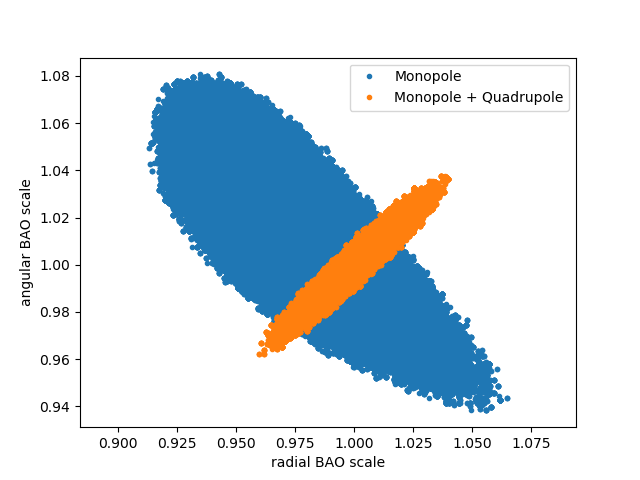
\includegraphics[width=0.48\textwidth]{prelimMCMC.png}
\end{center}
\end{wrapfigure}
The main outcome of this project will be the methods of extracting BAO/RSD
constraints from measured galaxy bispectrum. The main merit of this enterprise
is that these constraints will help to significantly tighten constraints on DE
and TG. DE is one of the biggest masteries in modern physics and for now our
only experimental handle on it is cosmological data. We have argued that the
even in the worst case scenario, in which systematics can only be controlled on
large scale, the results would still be helpful in tightening constraints on DE
and TG. In addition to this practical gain, the proper modeling of higher order
statistics of galaxy field would be interesting in itself. Nonlinearities in
gravitational evolution, bias, and RSD are difficult to model mathematically
and solving this problem would be a formidable intellectual achievement. The
results of the project will have practical application in other fields of
observational cosmology, including analysis of higher order clustering of weak
lensing, CMB and various cross-correlations.

\required{Broader Impacts}

While working on this project we will make a broader impact on society in
multiple complementary ways.

We will train a graduate student and a postdoc. The PhD student will be
involved in most aspects of this work and will gain invaluable experience in
data analysis, theoretical modeling of large-scale structure, and scientific
software development. The student will have an opportunity to get involved with
biggest cosmology surveys of next decade. By the end of the project the PhD
student will be in a very good position to pursue the research career in this
very promising field further and to contribute to the next generation of dark
energy experiments. The postdoc will also have an opportunity to work with DESI
and to produce a high impact work that will strongly enhance their career. The
PI and Co-PI will devote significant time to mentoring the PhD student and
postdoc.

As part of our project we plan to involve two undergraduate students in our
research activities. The students will help core team members in developing
software pipeline. This will be a wonderful opportunity for them to get
hands-on experience with scientific research and hone their programming,
physics, and mathematics skills. 

KSU cosmology group has a very good track record of involving undergraduate
students in research. PI has worked with four undergraduate students in last
three years. The Co-PI guides four to five undergraduates in cosmology
independent study each semester. In the last four years Co-PI submitted eight
papers with undergraduate students. A number of these students have been
accepted in good PhD programs. For instance, Sara Crandall is now at UC Santa
Cruz, Stephen Houston is at the University of Kansas, Drew Johnson joined the
PhD program at University of Minnesota, and Sanket Doshi and Varun Mathur just
joined the PhD programs at Maryland and Virginia. Both PI and Co-PI have been
active in the KSU REU program.

In addition we plan to run an extensive outreach program consisting of middle
and elementary school visits and public talks. The Co-PI and colleagues do about
an hour of physics demonstrations each year for the roughly 20 physics classes
in both the Manhattan Middle Schools, typically reaching over 450 eighth
graders each year. They have done this for the last eight years. They have also
put on a school-wide set of physics demonstrations each year at Theodore
Roosevelt Elementary, for more than 15 years. Typically, close to 300 students
and teachers see these demonstrations.

The Co-PI has organized many public lectures on science at KSU. These attract
large, diverse audiences that can include a number of upper elementary school
children and townies. On a number of occasions over 400 people have attended.
Last year John Preskill spoke about Quantum Computing and Fred Espenak (Mr.
Eclipse") talked about the Great American Total Solar Eclipse. The path of
totality was less than 100 miles from KSU and the PI, with other colleagues,
actively promoted this solar eclipse and KSU responded in a very positive
manner, allowing students to take ofrom classes on August 21 and arranging for
bus rides to two sites, one in NE Kansas (for 550 people!) and the other in NW
Missouri, both close to the path of totality.

Co-PI is a well-known public speaker on cosmology. He has spoken at many
Science Cafes, local observatories, planetaria, science museums, and amateur
astronomy clubs (including two of the largest, the St. Louis Astronomical
Society and the Astronomical Society of Kansas City), in the mid-west, across
the US, and internationally. A number of his talks have had audiences exceeding
150, one was attended by over 600 people.

PI and Co-PI plan to continue being involved in these rewarding outreach
activities.
